
\section{Evaluation}%
\label{sec:Evaluation}

\begin{figure}
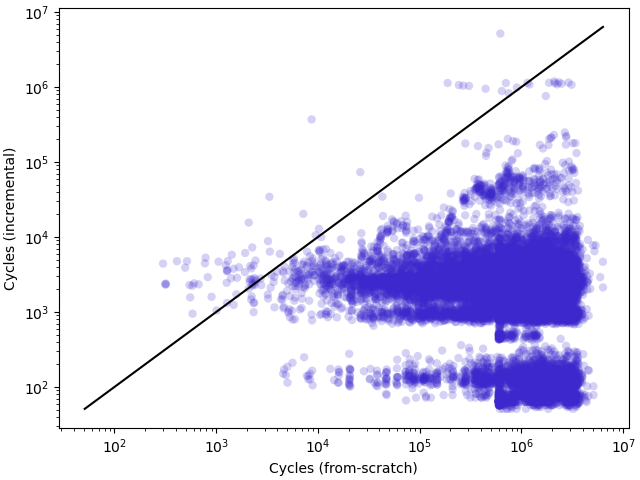
\includegraphics[width=0.75\linewidth]{images/scatter-plot.png}
\caption{Incremental vs. from-scratch editing times}
\label{fig:scatter-plot}
\end{figure}

%\label{sec:Evaluation}
%\begin{figure}
%\begin{minipage}{.48\linewidth}
%    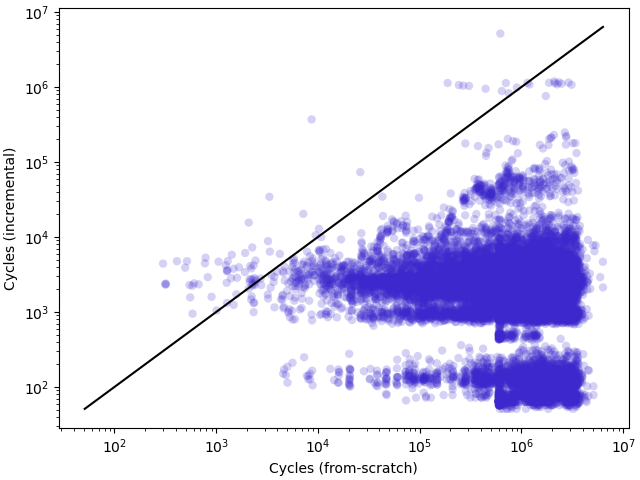
\includegraphics[width=\linewidth]{images/scatter-plot.png}
%    \caption{XXX}
%    \label{fig:scatter-plot}
%\end{minipage}
%\begin{minipage}{.48\linewidth}
%    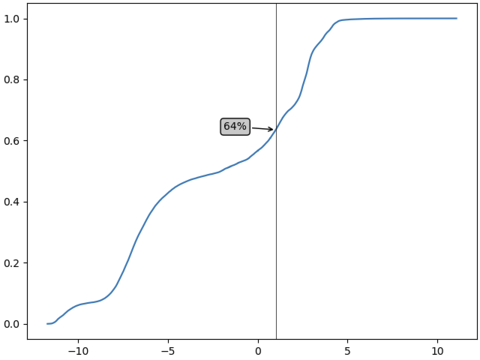
\includegraphics[width=\linewidth]{images/cdf.png}
%    \caption{YYY}
%    \label{fig:cdf}
%\end{minipage}
%\end{figure}

In this section we present our evaluation of the efficiency of Malcom relative to from-scratch type checking.  

\subsection{Benchmark}
We time Malcom on a synthesized edit trace constructed to test multiple aspects of Malcom. The first stage of the edit trace builds the program to a substantial size by constructing 100 nested copies of the merge sort algorithm. Each layer consists of a split function, a merge function, and a sort function. Each instance of the two helper functions, merge and split, is bound to a unique numbered identifier (\texttt{split\_n} and \texttt{merge\_n} for each layer \texttt{n}). Each sort function, on the other hand, is bound to the same identifier (\texttt{mergesort}). To capture long-distance binding patterns, each implementation of sort chooses which copy of split and which copy of merge to use uniformly at random from among those in scope. This  tests two aspects of Malcom's handling of bindings.

% The benchmark revolves around a `mergesort tower', a long chain of let-definitions, where the binding alternate between the options below:
% \begin{enumerate}
%     \item Binding a merge implementation to \texttt{merge\_n}, where \textsc{n} is the amount of previous merge definitions, to give each of them a unique name.
%     \item Binding a split implementation to \texttt{split\_n}.
%     \item Binding a mergesort implementation, which (at program construct time) randomly sample an available \texttt{merge\_n} and \textsc{split\_n} to depend on, to \texttt{mergesort}.
% \end{enumerate}
% Each of these options are defined and bounded to 100 times.

\begin{enumerate}
    \item \textbf{Shadowing}. Each \texttt{mergesort} shadows the one before it, testing Malcom's ability to find ancestor binders efficiently.
    \item \textbf{Name Reuse}. The definitions of \texttt{split\_n}, \texttt{merge\_n}, and \texttt{mergesort} each use common local variable names, such as \texttt{x}. Thus, those variable names are bound in multiple non-overlapping scopes, and Malcom must bind each occurrence to the correct binder.
    % \item \textbf{Irrelevant Names}. There are a multitude of different name, and name resolving should ignore irrelevant name, even though such names might change to shadow other variables in the future.
\end{enumerate}

The edit trace builds this tower by inserting constructors at leaves of the program sketch until complete. At each point in construction, the children of the current node in the sketch are constructed in a random order, and this proceeds recursively. This randomness ensures that different patterns of variable interactions are tested: for example, a variable binding might be inserted into an abstraction after its body has been constructed, capturing the free occurrences in the body.
% The program is built up randomly and recursively: to build a tree \textbf{X} at a Hole, the editor replace the hole with the root node of \textbf{X}, but with all children being empty Hole. It then randomly select a children which is not instantiated yet (so a hole), move down into it build it, and move up, repeating this process until all children had been instantiated. The randomness ensures different kinds of variable interactions are tested: for example, a variable binding might be inserted in the middle of the tree, thus shadowing the same binding from its ancestor, and being shadowed by the same binding from its descendents.

After the construction phase of the edit trace, random edits are applied throughout the program. Each of these edit sequences consists of moving to a uniformly random location in the program, applying a small change based on the node, and reverting the change. This is repeated 500 times. The changes include:
% After the program is built up, we apply random edits to the tree by selecting a random location, moving to the location, applying some small changes to the tree, and reverting our changes. The changes we apply includes:
\begin{enumerate}
    \item Deleting a leaf node and inserting another in its place.
    \item Replacing a binder with another.
    \item Wrapping a constructor around a subterm.
    \item Alternatively, for constructors with one child subexpression (for which unwrapping does not delete subexpressions), unwrapping the constructor.
\end{enumerate}
% \begin{enumerate}
%     \item Deleting an atom to insert an atom in its place, as the most basic 'incremental check'.
%     \item Deleting a binder and insert an existing binder to stress shadowing resolution.
%     \item Wrapping a Node with an unwrapping the node
%     \item Alternatively, if the Node have one children, so unwrapping will not lose information, unwrapping the node then wrapping it again to revert.
% \end{enumerate}
These edits test deletion, insertion, wrapping, and unwrapping, including updating types and binders. They also can introduce errors, demonstrating Malcom's incremental error marking ability.

\subsection{Results}
For each non-move edit, we measure the time it takes to perform the action and propagate updates until quiescent. Timing is done with \texttt{rdtsc}. For a baseline, the same edit is performed on a bare syntax tree represented with a zipper data structure, and is type checked from scratch according to the ordinary MALC marking procedure. The total time to edit and type check is compared between the incremental and from-scratch analyses. Note that action performance can be slower for Malcom than for the ordinary zipper representation, since Malcom computes changes to bindings at edit time. Figure \ref{fig:scatter-plot} show a scatter plot comparing these times (in cycles) for Malcom and the from-scratch analysis. Each data point is one non-move edit to the program. Points above the diagonal (shown in black)  are edits where the from-scratch analysis is faster than the incremental one, and below the diagonal is the converse. Almost all points are below the diagonal, meaning that incrementality provides a speedup in almost all cases. Many points are far below the diagonal, with incrementality providing one or more orders of magnitude of speedup. The data points are multi-modal, forming multiple horizontal bands. This indicates a fundamental algorithmic speedup: while the from-scratch analysis grows linearly in program size, empirically the incremental analysis shows hardly any growth. The horizontal bands are likely made up of different kinds of actions. The top-most band displays a slight positive trend, indicating cases where the incremental analysis does grow with the program size. This band likely contains edits that affect binding structure.

In total across all of these edits, Malcom provides whopping \speedup speedup over from-scratch marking, demonstrating its substantial advantage over non-incremental analysis in providing continuous static feedback.